\documentclass[french]{beamer}
\usepackage{hyperref}
\usepackage[T1]{fontenc}
\usepackage{lmodern}
\usepackage{listings}
\usepackage{pgfplots}  

% \UseRawInputEncoding

% Cannot enable in Xelatex
\usepackage{pgfpages}
% \setbeameroption{hide notes} % Only slides
% \setbeameroption{show only notes} % Only notes
% \setbeameroption{show notes on second screen}

% other packages
\usepackage{latexsym,amsmath,xcolor,multicol,booktabs,calligra}
\usepackage{graphicx,listings,stackengine}

%% Enable only in Xelatex
% \usepackage{pstricks}

\author{Charles Perry}
\title{La sémantique par valeur revisitée}
\subtitle{Une approche C++ moderne}
\institute {Savoir-Faire Linux}
\usepackage{SFL}

% defs
\def\cmd#1{\texttt{\color{red}\footnotesize $\backslash$#1}}
\def\env#1{\texttt{\color{blue}\footnotesize #1}}
\definecolor{deepblue}{rgb}{0,0,0.5}
\definecolor{deepred}{rgb}{0.6,0,0}
\definecolor{deepgreen}{rgb}{0,0.5,0}
\definecolor{halfgray}{gray}{0.55}

\lstset{language=C++,
                basicstyle=\small,
                keywordstyle=\color{blue}\ttfamily,
                stringstyle=\color{red}\ttfamily,
                commentstyle=\color{deepgreen}\ttfamily,
                morecomment=[l][\color{magenta}]{\#}
}
\hypersetup{
    colorlinks=true,
    linkcolor=blue,
    filecolor=magenta,      
    urlcolor=cyan,
    pdftitle={Overleaf Example},
    pdfpagemode=FullScreen,
    }

\begin{document}

\begin{frame}
    \titlepage
%    \begin{figure}[htpb]
%        \begin{center}
%            \includegraphics[width=0.2\linewidth]{pic/YTU_logo.jpg}
%        \end{center}
%    \end{figure}

\end{frame}

\begin{frame}{À propos du présentateur}
    \begin{minipage}{0.4\linewidth}
    \begin{figure}
        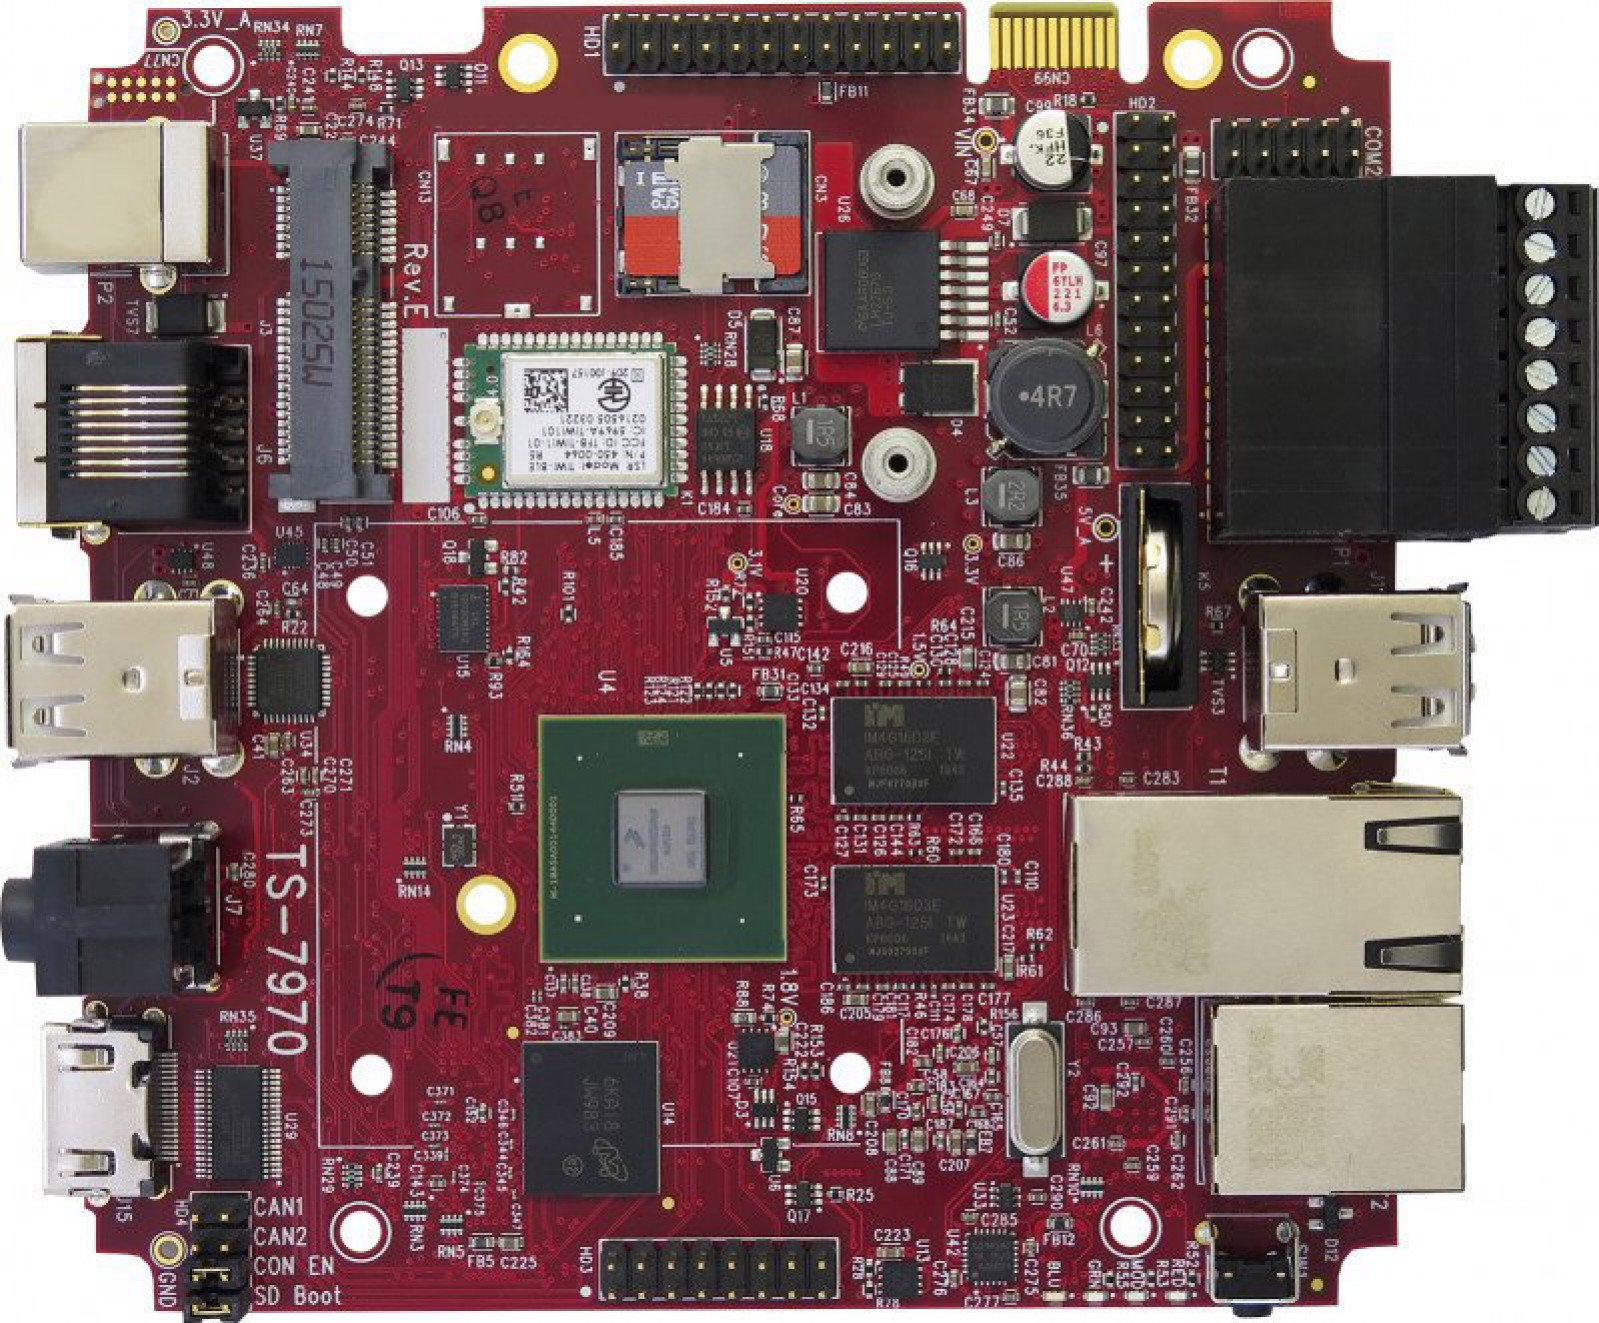
\includegraphics[width=\linewidth]{intro_pcb.jpg}
    \end{figure}
    \end{minipage}
    \begin{minipage}{0.58\linewidth}
        Équipe ingénierie produit:
        \begin{itemize}
            \item Intégration des composant logiciels dans une plateforme embarquée
            \item Intégration du noyau Linux et développement de pilotes
            \item Développement d'applications
            \item Et bien plus!
        \end{itemize}
    \end{minipage}
\end{frame}

\begin{frame}{À propos de la présentation}
    \begin{minipage}{0.3\linewidth}
    \begin{figure}
        
\includegraphics[width=\linewidth]{cppcon.png}
    \end{figure}
    \end{minipage}
    \begin{minipage}{0.68\linewidth}
        \begin{itemize}
            \item Matériel original: "Back To Basics: Value Semantics" par Klaus Iglberger (Cppcon 2022)
            \item Disponnible sur \href{https://github.com/CppCon/CppCon2022/blob/main/Presentations/Back-to-Basics-Value-Semantics-Klaus-Iglberger-CppCon-2022.pdf}{github}
        \end{itemize}
    \end{minipage}
\end{frame}

\begin{frame}{Un peu d'histoire: Bjarne Stroustrup}
    \begin{minipage}{0.5\linewidth}
    \begin{figure}
        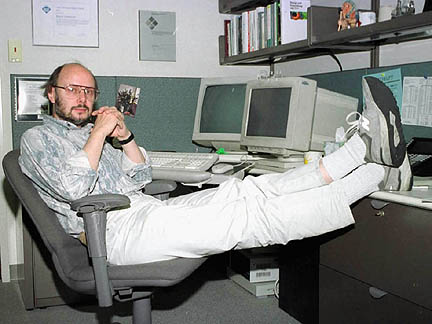
\includegraphics[width=\linewidth]{BjarneStroustrup.jpg}
    \end{figure}
    \end{minipage}
    \begin{minipage}{0.48\linewidth}
        \begin{itemize}
            \item 1979: Utilise simula dans sa thèse de doctorat intitulée "Communication and control in distributed computer systems"
            \item 1979: Rejoint le laboratoire Bell au New Jersey ("Bell Labs")
            \item 1985: C++ est disponible au grand public
        \end{itemize}
    \end{minipage}
\end{frame}

\begin{frame}{Un peu d'histoire}
    \begin{figure}
        
\includegraphics[width=\linewidth]{c_simula.png}
    \end{figure}
\end{frame}

\begin{frame}{Design Patterns - 1994}
    \begin{minipage}{0.4\linewidth}
    \begin{figure}
        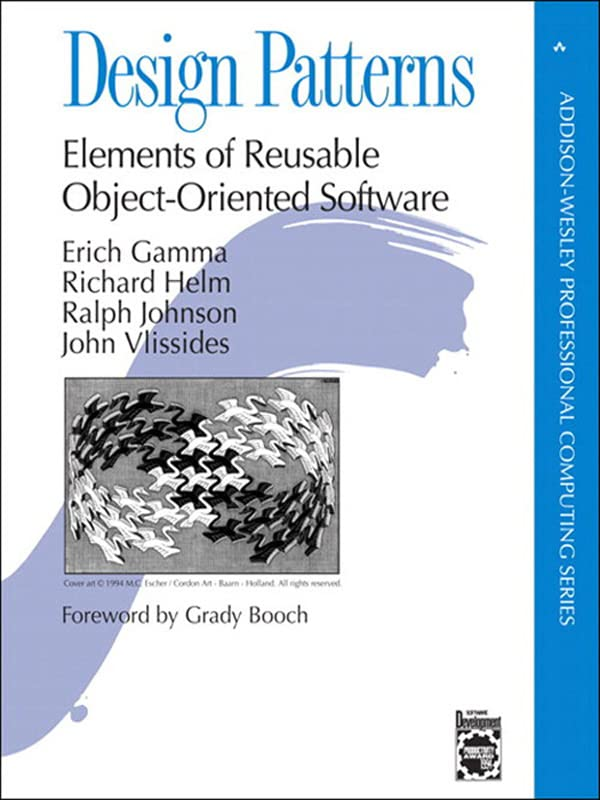
\includegraphics[width=\linewidth]{gof_book.jpg}
    \end{figure}
    \end{minipage}
    \begin{minipage}{0.5\linewidth}
        \begin{itemize}
            \item Livre du "Gang of four"
            \item Publié en 1994
            \item Jette les bases de 23 "design patterns" utilisant le principe de programmation orientée objet (POO).
            \item Tous les "design patterns" reposent sur le principe d'héritage.
        \end{itemize}
    \end{minipage}
\end{frame}

\begin{frame}{Visiteur}
    \begin{figure}
        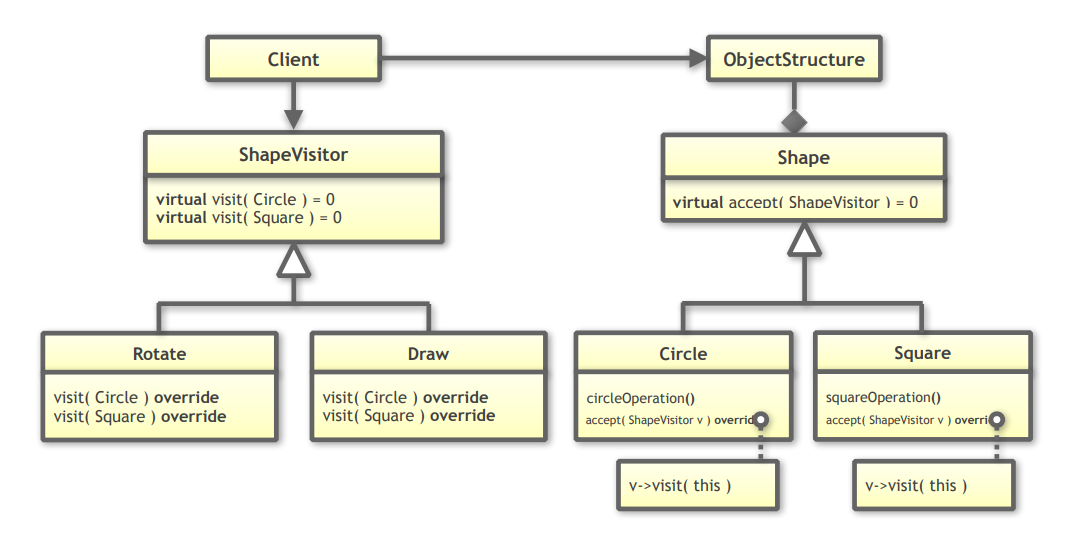
\includegraphics[width=\linewidth]{visitor.png}
    \end{figure}
\end{frame}

\begin{frame}{Exemple: dessiner des formes}
    \begin{figure}
        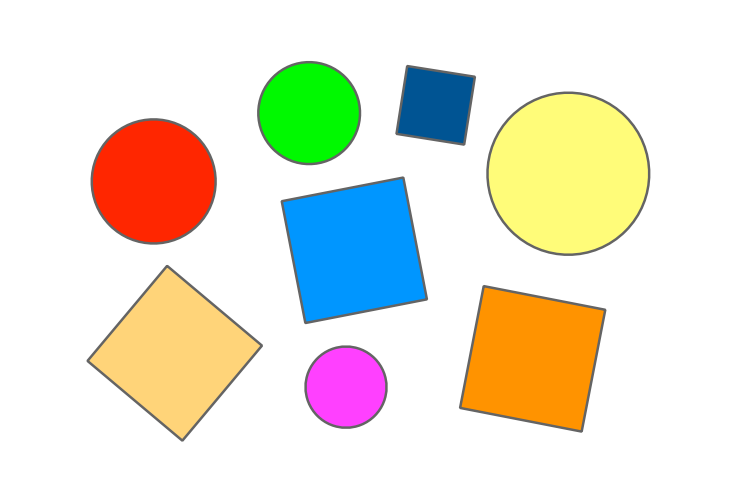
\includegraphics[width=0.8\linewidth]{formes.png}
    \end{figure}
\end{frame}

\begin{frame}[fragile]{Dessiner des formes: POO classique}
    \begin{lstlisting}[language=C++]
class Circle;
class Square;

class ShapeVisitor
{
public:
  virtual ~ShapeVisitor() = default;
  virtual void visit( const Circle& ) const = 0;
  virtual void visit( const Square& ) const = 0;
};
    \end{lstlisting}
\end{frame}

\begin{frame}[fragile]{Dessiner des formes: POO classique}
    \begin{lstlisting}[language=C++]
class Shape
{
public:
  Shape() = default;
  virtual ~Shape() = default;

  virtual void accept( const ShapeVisitor& ) = 0;
};
    \end{lstlisting}
\end{frame}

\begin{frame}[fragile]{Dessiner des formes: POO classique}
    \begin{lstlisting}[language=C++]
class Circle : public Shape
{
public:
  explicit Circle( double rad, /* ... */ )
    : radius_{ rad }, /* ... */
    {}
 
  double getRadius() const;
  // ... getCenter(), getRotation(), ...

  void accept( const ShapeVisitor& ) override;
 
private:
  double radius_;
  /* ... */
};
    \end{lstlisting}
\end{frame}

\begin{frame}[fragile]{Dessiner des formes: POO classique}
    \begin{lstlisting}[language=C++]
class Square : public Shape
{
public:
  explicit Square( double s, /* ... */ )
    : side_{ s }, /* ... */
    {}
 
  double getSide() const;
  // ... getCenter(), getRotation(), ...

  void accept( const ShapeVisitor& ) override;
 
private:
  double side_;
  /* ... */
};
    \end{lstlisting}
\end{frame}

\begin{frame}[fragile]{Dessiner des formes: POO classique}
    \begin{lstlisting}[language=C++]
class Draw : public ShapeVisitor
{
public:
  void visit( const Circle& ) const override;
  void visit( const Square& ) const override;
};
    \end{lstlisting}
\end{frame}

\begin{frame}[fragile]{Dessiner des formes: POO classique}
    \begin{lstlisting}[language=C++]
void drawAllShapes(
  const std::vector<std::unique_ptr<Shape>>& shapes)
{
  for(const auto& s : shapes)
  {
    s->accept(Draw{})
  }
}
    \end{lstlisting}
\end{frame}

\begin{frame}[fragile]{Dessiner des formes: POO classique}
    \begin{lstlisting}[language=C++]
int main()
{
  using Shapes = std::vector<std::unique_ptr<Shape>>;
 
  Shapes shapes;
  shapes.emplace_back(std::make_unique<Circle>( 2.0 ));
  shapes.emplace_back(std::make_unique<Square>( 1.5 ));
  shapes.emplace_back(std::make_unique<Circle>( 4.2 ));
 
  drawAllShapes(shapes);
}
    \end{lstlisting}
\end{frame}

\begin{frame}{Désavantages de l'approche POO classique}
    Le design POO classique a plusieurs désavantages:
    \begin{itemize}
        \item Deux hiérarchies de classes (intrusif).
        \item Deux appels de fonction virtuelle par opération (performance).
        \item Nécessite d'accéder aux objets via un pointeur (complexité accidentelle).
        \item Plusieurs allocations dynamiques petites (performance).
        \item Gestion manuelle de la mémoire (prompt aux erreurs).
    \end{itemize}
\end{frame}

\begin{frame}[fragile]{std::variant contre-attaque}
    \begin{figure}
        
\includegraphics[width=0.7\linewidth]{yoda.jpg}
    \end{figure}
    \begin{lstlisting}[language=C++, basicstyle=\normalsize]
using Shapes = std::variant<Circle, Square>;
    \end{lstlisting}
\end{frame}

\begin{frame}[fragile]{std::variant?}
    \begin{itemize}
        \item Introduit avec C++17
        \item Représente une valeur d'une liste de type (one of).
        \item Type-safe \lstinline{union}
        \item Pas d'allocation dynamique.
    \end{itemize}
    \begin{lstlisting}[language=C++]
class std::variant<int, float, double>
{
    union {
        int a;
        float b;
        double c;
    } value_;
    int active_;
public:
    /* ... */
}
    \end{lstlisting}
\end{frame}

\begin{frame}[fragile]{Dessiner des formes: Sémantique par valeur}
    \begin{lstlisting}[language=C++]
class Circle
{
public:
  explicit Circle( double rad, /* ... */ )
    : radius_{ rad }, /* ... */
    {}
 
  double getRadius() const;
  // ... getCenter(), getRotation(), ...
 
private:
  double radius_;
  /* ... */
};
    \end{lstlisting}
\end{frame}

\begin{frame}[fragile]{Dessiner des formes: Sémantique par valeur}
    \begin{lstlisting}[language=C++]
class Square
{
public:
  explicit Square( double s, /* ... */ )
    : side_{ s }, /* ... */
    {}
 
  double getSide() const;
  // ... getCenter(), getRotation(), ...
 
private:
  double side_;
  /* ... */
};
    \end{lstlisting}
\end{frame}

\begin{frame}[fragile]{Dessiner des formes: Sémantique par valeur}
    \begin{lstlisting}[language=C++]
class Draw
{
public:
  void operator()( const Circle& ) const;
  void operator()( const Square& ) const;
};
    \end{lstlisting}
\end{frame}

\begin{frame}[fragile]{Dessiner des formes: Sémantique par valeur}
    \begin{lstlisting}[language=C++]
using Shape = std::variant<Circle, Square>;

void drawAllShapes(
  const std::vector<Shape>& shapes)
{
  for(const auto& s : shapes)
  {
    std::visit(Draw{}, s);
  }
}
    \end{lstlisting}
\end{frame}

\begin{frame}[fragile]{Dessiner des formes: Sémantique par valeur}
    \begin{lstlisting}[language=C++]
int main()
{
  using Shapes = std::vector<Shape>;
 
  Shapes shapes;
  shapes.emplace_back( Circle( 2.0 ) );
  shapes.emplace_back( Square( 1.5 ) );
  shapes.emplace_back( Circle( 4.2 ) );
 
  drawAllShapes(shapes);
}
    \end{lstlisting}
\end{frame}

\begin{frame}{Avantages de l'approche par valeur}
    Le design par valeur a plusieurs avantages:
    \begin{itemize}
        \item Aucune hiérarchie de classe (non-intrusif).
        \item Aucun appel de fonction virtuelle (performance).
        \item Plus besoin d'accéder aux objets via un pointeur (simplicité).
        \item Aucune allocation dynamique (performance).
        \item Aucune gestion manuelle de la mémoire (simplicité).
    \end{itemize}
\end{frame}

\begin{frame}[fragile]{std::visit ???}
    \begin{figure}
        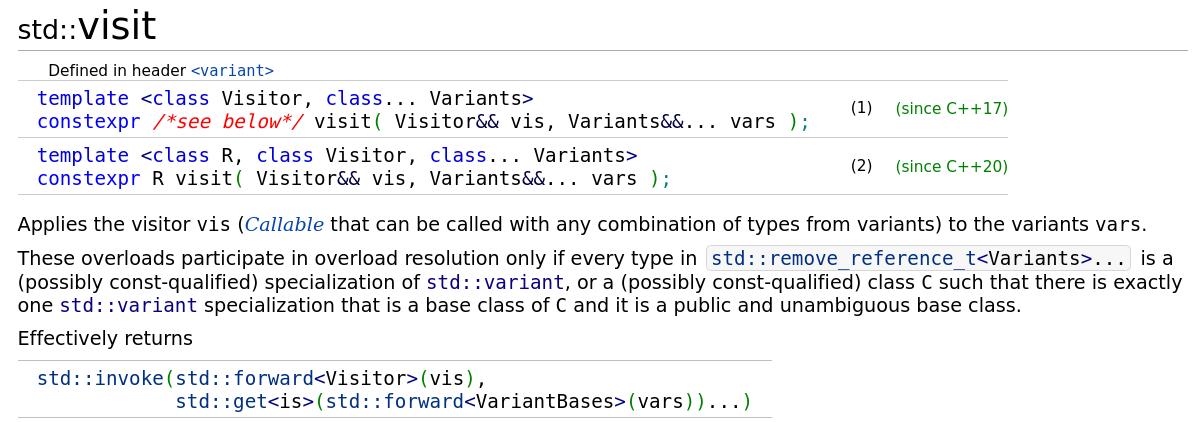
\includegraphics[width=\linewidth]{visit.png}
    \end{figure}
\end{frame}

\begin{frame}[fragile]{Performance}
    \begin{itemize}
        \item À titre qualitatif seulement, les résultats peuvent varier.
        \item Compiler avec \lstinline{-O1} minimalement.
    \end{itemize}
\end{frame}

\begin{frame}[fragile]{Performance}
    \begin{itemize}
        \item 1 millions de formes.
        \item GCC 11.3
        \item Utilisation de google/benchmark pour mesurer le temps CPU et assurer la convergence.
        \item Intel Core i7-4770 CPU @ 3.40GHz
        \item Cache:
        \begin{itemize}
            \item 32 KiB L1 Data
            \item 32 KiB L1 Instruction
            \item 256 KiB L2
            \item 8 MiB L3
        \end{itemize}
    \end{itemize}
\end{frame}

\begin{frame}[fragile]{Performance}
    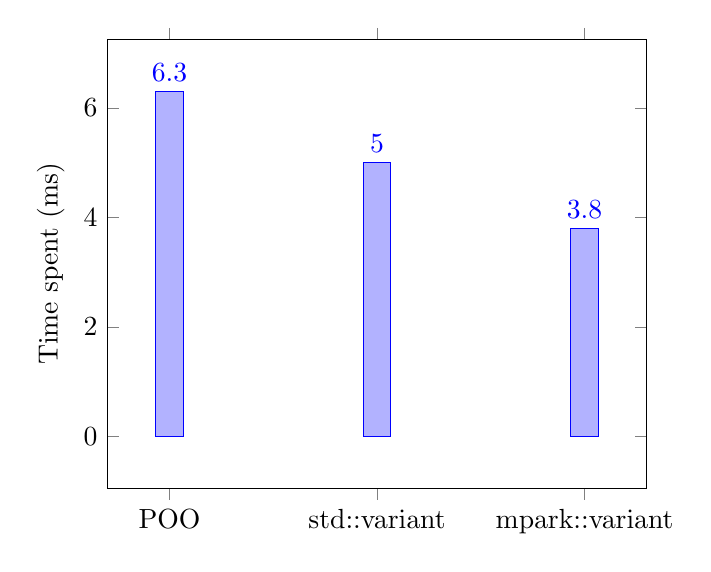
\begin{tikzpicture}  
    \begin{axis}
    [  
        ybar,
        ymin=0,
        enlargelimits=0.15,  
        ylabel={Time spent (ms)}, % the ylabel must precede a # symbol.  
        xlabel={},  
        symbolic x coords={POO, std::variant, mpark::variant}, % these are the specification of coordinates on the x-axis.  
        xtick=data,  
         nodes near coords, % this command is used to mention the y-axis points on the top of the particular bar.  
        nodes near coords align={vertical},  
        ]  
    \addplot coordinates {(POO,6.3) (std::variant,5.0) (mpark::variant,3.8) };  
      
    \end{axis}  
    \end{tikzpicture}  
\end{frame}

\begin{frame}[fragile]{Exemple #2: exactitude du mot clé const}
    \begin{lstlisting}[language=C++]
void print(const std::vector<int>& vec);

int main()
{
  std::vector<int> v{1,2,3,4};
  
  const std::vector<int> w{ v };
  const std::span<int> s{ v };
  
  w[2] = 99; // Compilation error!
  s[2] = 99; // Ok!
  
  print( v );
}
    \end{lstlisting}
\end{frame}

\begin{frame}[fragile]{Exemple #2: exactitude du mot clé const}
    \begin{lstlisting}[language=C++]
void print(const std::vector<int>& vec);

int main()
{
  std::vector<int> v{1,2,3,4};
  
  const std::vector<int> w{ v };
  const std::span<const int> s{ v };
  
  w[2] = 99; // Compilation error!
  s[2] = 99; // Compilation error!
  
  print( v );
}
    \end{lstlisting}
\end{frame}

\begin{frame}{Exactitude du mot clé const}
    Le mot clé \lstinline{const} peut prendre différents sens avec une sémantique de référence, ce qui n'est pas le cas avec la sématique par valeur.
    \begin{itemize}
        \item Un pointeur: \lstinline{const int* const}
        \item Un span: \lstinline{const std::span<const int>}
        \item Pour un type à sémantique par valeur, \lstinline{const} veut dire \lstinline{const}! Par exemple: \lstinline{const std::vector<std::vector<std::string>>} ne permet pas de modifier le moindre caractère.
    \end{itemize}
\end{frame}

\begin{frame}[fragile]{Exemple #3: problèmes d'invalidation}
    \begin{lstlisting}[language=C++]
void print(std::span<int> s);

int main()
{
  std::vector<int> v{1,2,3,4};
  
  const std::span<int> s{ v };
  
  print( s ); // Ok
  
  v = {5,6,7,8,9}; // s is invalidated here
  
  print( s ); // Undefined behavior
}
    \end{lstlisting}
\end{frame}

\begin{frame}[fragile]{Exemple #4: problèmes d'invalidation}
    \begin{lstlisting}[language=C++]
void print(std::span<const int> s);

int main()
{
  std::vector<int> v{1, -3, 42, 4, -8, 22, 42, 37, 4,9};
  
  print(v); // 1, -3, 42, 4, -8, 22, 42, 37, 4, 9
  
  const auto pos = std::max_element(begin(v), end(v));
  
  v.erase(std::remove(begin(v), end(v), *pos), end(v));
  
  print(v); // 1, -3, 4, -8, 22, 42, 37, 9
}
    \end{lstlisting}
\end{frame}

\begin{frame}[fragile]{Exemple #4: problèmes d'invalidation}
    \begin{figure}
        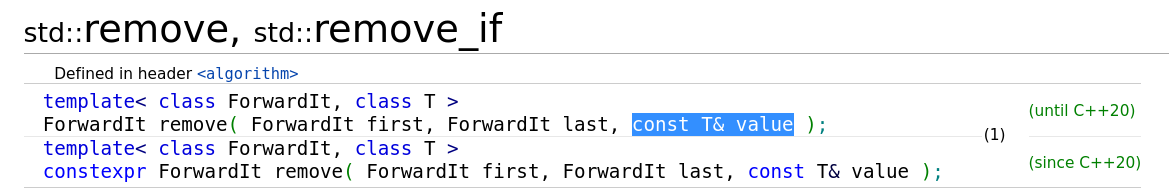
\includegraphics[width=1.1\linewidth]{remove.png}
    \end{figure}
\end{frame}

\begin{frame}{Problèmes d'invalidation}
    \begin{itemize}
        \item La plupart des problèmes d'invalidation surviennent lorsqu'une référence est utilisé trop longtemps.
        \item En règle général, passer un argument par référence ne pose pas problème. Toutefois, retourner d'une fonction par référence peut poser problème.
    \end{itemize}
\end{frame}

\begin{frame}[fragile]{Exemples de types à sémantique...}
    \begin{minipage}{0.45\linewidth}
        ... par valeur
        \begin{itemize}
            \item \lstinline{std::vector} et tous les conteneurs de la STL (C++98)
            \item \lstinline{std::function} (C++11)
            \item \lstinline{std::variant} (C++17)
            \item \lstinline{std::optional} (C++17)
            \item \lstinline{std::expected} (C++23)
        \end{itemize}
    \end{minipage}
    \begin{minipage}{0.45\linewidth}
        ... par référence
        \begin{itemize}
            \item \lstinline{T&}
            \item \lstinline{T*}
            \item \lstinline{std::span}
            \item \lstinline{std::string_view}
            \item \lstinline{std::unique_ptr}
            \item \lstinline{std::shared_ptr}
            \item \lstinline{std::iterator} et autres itérateurs
        \end{itemize}
    \end{minipage}
\end{frame}

\begin{frame}[fragile]{Caractéristiques de la sémantique...}
    \begin{minipage}{0.45\linewidth}
        ... par valeur
        \begin{itemize}
            \item Copie profonde (deep copy)
            \item \lstinline{const} se propage
        \end{itemize}
    \end{minipage}
    \begin{minipage}{0.45\linewidth}
        ... par référence
        \begin{itemize}
            \item Copie superficielle (shallow copy)
            \item \lstinline{const} ne se propage pas
        \end{itemize}
    \end{minipage}
\end{frame}

\begin{frame}{Conclusion}
    Lorsque possible, préférer la sémantique par valeur à la sémantique par référence. Votre code en sera:
    \begin{itemize}
        \item plus facile à comprendre
        \item plus facile à écrire
        \item plus facile à maintenir
        \item potentiellement plus rapide
    \end{itemize}
\end{frame}

\end{document}